\documentclass{article}
\usepackage[top=2.5cm, bottom=2.5cm, left=2cm, right=2cm]{geometry}
\usepackage{amsmath} 
\usepackage{amssymb}
\usepackage{mathrsfs}
\usepackage{amscd}
\usepackage{graphicx} 
\usepackage{subfig} 
\usepackage{tabularx}
\usepackage{indentfirst} 
\usepackage{array}
\usepackage{longtable}
\usepackage{multirow}
\usepackage{bm}
\usepackage{cite}
\usepackage{enumerate}


\author{Wang Dongying}
\title{Reflectivity vs incident angle}
\begin{document}
\maketitle

	When light is reflected or transmitted by samples at oblique incidence, the light is classified into p- and s-polarized light waves depending on the oscillatory direction of its electric field and each light wave shows quite different behavior. In p-polarization, the electric fields of incident and reflected light waves oscillatewithin the same plane. This particular plane is called the plane of incidence. The boundary conditions for electromagnetic waves require the parallel components on the incident side must be equal to that on the transmission side.\\

	In this case, I only consider the electrical field $E$. The material has the dieletric constant $\epsilon_{A} = \epsilon_{1,A} + i\epsilon_{2,A}$, where the complex refractive index $N_{A} = \sqrt{\epsilon_{A}}$.

	\section{Boundary conditions of electrical field}

		\begin{equation}
		\begin{aligned}
			E_{1\tau} - E_{2\tau} = 0\\
			D_{1n} - D_{2n} = 0
		\end{aligned}
		\end{equation}

		where $\bm{D} = \epsilon\bm{E}$.

	\section{Reflectivity of p-polarized light}
		I consider it is a material bulk in the environment of air, which the refractive index and dielectric constant sets to 1, for convinience. Snell's law is expressed as
		\begin{equation}
			sin\theta_{i} = N_{A}sin\theta_{t}
		\end{equation}

		Using the boundary conditions of electrical field. Got these

		\begin{equation}
		\begin{aligned}
			E_{ip}sin\theta_{i} + E_{rp}sin\theta_{r} = \epsilon_{A}E_{tp}sin\theta_{t}\\
			E_{ip}cos\theta_{i} - E_{rp}cos\theta_{r} = E_{tp}cos\theta_{t}	
		\end{aligned}
		\end{equation}

		By solving these two equations, 
		\begin{equation}
			r_{p} = \frac{E_{rp}}{E_{ip}} = \frac{N_{A}cos\theta_{i} - cos\theta_{t}}{N_{A}cos\theta_{i} + cos\theta_{t}} = \frac{\epsilon_{A}cos\theta_{i} - (\epsilon_{A} - sin^{2}\theta_{i})^{1/2}}{\epsilon_{A}cos\theta_{i} + (\epsilon_{A} - sin^{2}\theta_{i})^{1/2}}
		\end{equation}

		And then, the reflectivity can be expressed as 

		\begin{equation}
			R_{p} = |r_{p}|^{2}
		\end{equation}

	\section{Reflectivety of s-polarized light}

		Because of the direction, we could only have one function according to boundary condition of electrical field.
		\begin{equation}
			E_{is} + E_{rs} = E_{ts}
		\end{equation}

		So we should use the one for magnetic field. Notice that in the medium, $E = \frac{c}{N_{A}}B$.
		\begin{equation}
			-B_{is}cos\theta_{i} + B_{rs}cos\theta_{r} = -B_{ts}cos\theta_{t}
		\end{equation}

		By solving these two equations, 
		\begin{equation}
			r_{s} = \frac{E_{rs}}{E_{is}} = \frac{cos\theta_{i} - (\epsilon_{A} - sin^{2}\theta_{i})^{1/2}}{cos\theta_{i} + (\epsilon_{A} - sin^{2}\theta_{i})^{1/2}}
		\end{equation}		

		And then, the reflectivity can be expressed as 

		\begin{equation}
			R_{p} = |r_{p}|^{2}
		\end{equation}


		\begin{figure}
		\centering
			\begin{minipage}[b]{0.45\linewidth}
			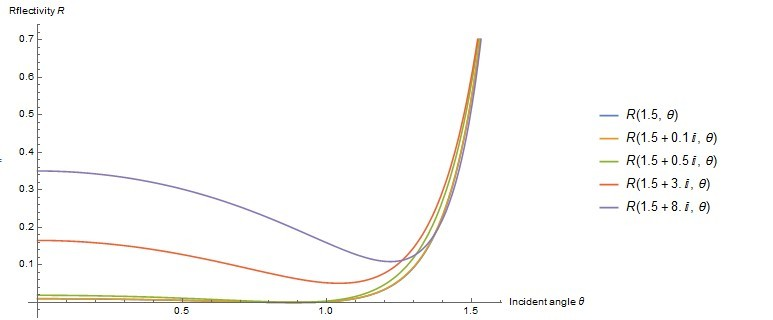
\includegraphics[width=\linewidth]{fig1.jpg}
			\caption{$R_{p}$ vs $\theta$ with different $\epsilon_{2,A}$}
			\label{fig:minipage1}
			\end{minipage}
			\quad
			\begin{minipage}[b]{0.45\linewidth}
			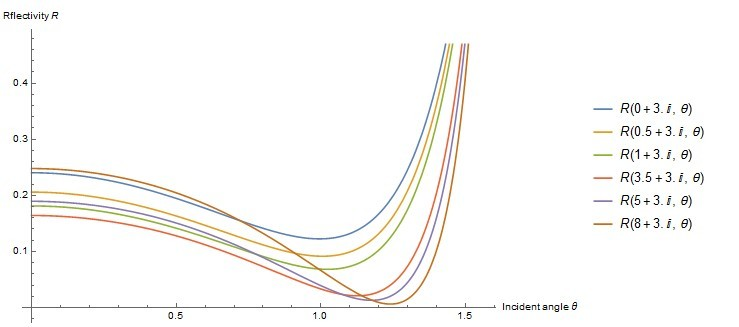
\includegraphics[width=\linewidth]{fig2.jpg}
			\caption{$R_{p}$ vs $\theta$ with different $\epsilon_{1,A}$}
			\label{fig:minipage2}
			\end{minipage}
		\end{figure}

		\begin{figure}
		\centering
			\begin{minipage}[b]{0.45\linewidth}
			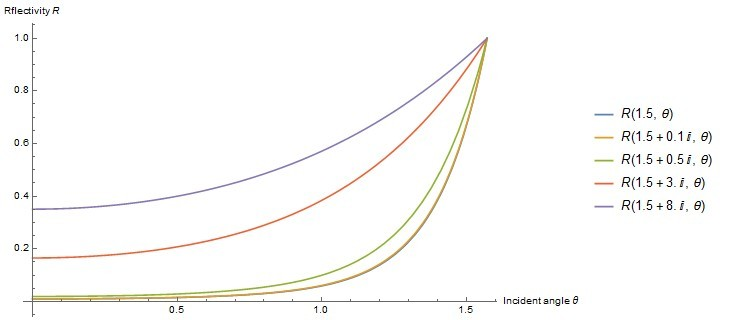
\includegraphics[width=\linewidth]{fig3.jpg}
			\caption{$R_{s}$ vs $\theta$ with different $\epsilon_{2,A}$}
			\label{fig:minipage1}
			\end{minipage}
			\quad
			\begin{minipage}[b]{0.45\linewidth}
			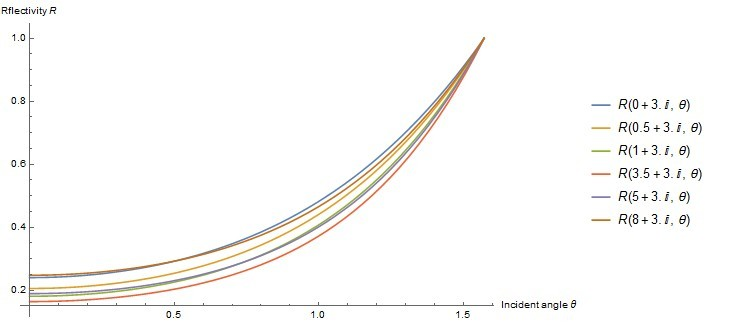
\includegraphics[width=\linewidth]{fig4.jpg}
			\caption{$R_{s}$ vs $\theta$ with different $\epsilon_{1,A}$}
			\label{fig:minipage2}
			\end{minipage}
		\end{figure}

	\section{Bragg diffraction}

		
		Bragg's law describes the condition on θ for the constructive interference to be at its strongest:

		\begin{equation}
			n\lambda = 2dsin\theta
		\end{equation}

		Considering that the photon has energy of $530eV$ and the lattice constant of medium is $20\AA$. The angle of Bragg diffraction can be calculated.

		\begin{equation}
			\theta = arcsin(\frac{n\lambda}{2d}) = arcsin(\frac{nch}{2dE}) = 0.626rad
		\end{equation}

		There will be a sharp diffraction peak at 0.626rad.




\end{document}